%%%%%%%%%%%%%%%%%%%% LANChat-H camera-ready copy (Springer svmult chapter) %%%%%%%%%%%%%%%%%%%%
\documentclass[graybox]{svmult}

\usepackage{type1cm}
\usepackage{graphicx}
\usepackage[bottom]{footmisc}
\usepackage{newtxtext}
\usepackage{newtxmath}
\usepackage{url}
\usepackage{array}

\newcommand{\code}[1]{\texttt{#1}}
\newcommand{\lch}{\mbox{LANChat-H}}
\setcounter{topnumber}{3}\setcounter{totalnumber}{4}
\renewcommand{\topfraction}{0.9}\renewcommand{\bottomfraction}{0.9}
\renewcommand{\textfraction}{0.1}\renewcommand{\floatpagefraction}{0.7}
\raggedbottom

\begin{document}

\title*{LANChat-H: Design, Implementation and Evaluation of a Dependency-Light Secure LAN Chat System with End-to-End Encryption}
\titlerunning{LANChat-H: a Secure LAN Chat System with End-to-End Encryption}
\author{Harish Goud B and Revanth Reddy Lingala and Saarthak Manocha*}
\authorrunning{H. Goud B et al.}
\institute{Harish Goud B \at Chaitanya Bharathi Institute of Technology, Hyderabad, Telangana, India,\\ \email{harishgoudbit@cbit.ac.in}
\and Revanth Reddy Lingala \at Chaitanya Bharathi Institute of Technology, Hyderabad, Telangana, India,\\ \email{revanthreddy0906@gmail.com}
\and Saarthak Manocha* \at Chaitanya Bharathi Institute of Technology, Hyderabad, Telangana, India,\\ \email{saarthakmanocha10@gmail.com}\\[2pt]
* Corresponding author}
\maketitle

\abstract*{Small teams and classrooms often want a private chat that stays on their own network, but the usual options are either heavy or lack identity, persistence and protection from whoever runs the server. We present \lch{}, a LAN chat system whose core uses only the Python standard library. It combines length-prefixed TCP framing with a plain-text fallback, a bounded outbound queue per client that isolates slow receivers, TLS with trust-on-first-use pinning, memory-hard credentials with lockout and rate limits, roles, SQLite persistence, ticketed file transfer and a hash-chained audit log. End-to-end encryption (X25519, Ed25519, ChaCha20-Poly1305) covers private messages, files and an optional group room, so the server stores only ciphertext. The limits are stated up front: no forward secrecy, visible metadata, and trust only as good as the comparison of security codes. In repeated loopback trials with 100 receivers the median delivery time was 6.9 ms for \lch{} and 2.3 ms for an asyncio relay; a stalled receiver stopped a sequential relay after 232 messages but not \lch{}; and a mixed workload through an emulated network path added about 7 ms to the path delay. Our own fuzzing found and fixed one real bug; it is not an independent audit.}

\abstract{Small teams and classrooms often want a private chat that stays on their own network, but the usual options are either heavy or lack identity, persistence and protection from whoever runs the server. We present \lch{}, a LAN chat system whose core uses only the Python standard library. It combines length-prefixed TCP framing with a plain-text fallback, a bounded outbound queue per client that isolates slow receivers, TLS with trust-on-first-use pinning, memory-hard credentials with lockout and rate limits, roles, SQLite persistence, ticketed file transfer and a hash-chained audit log. End-to-end encryption (X25519, Ed25519, ChaCha20-Poly1305) covers private messages, files and an optional group room, so the server stores only ciphertext. The limits are stated up front: no forward secrecy, visible metadata, and trust only as good as the comparison of security codes. In repeated loopback trials with 100 receivers the median delivery time was 6.9 ms for \lch{} and 2.3 ms for an asyncio relay; a stalled receiver stopped a sequential relay after 232 messages but not \lch{}; and a mixed workload through an emulated network path added about 7 ms to the path delay. Our own fuzzing found and fixed one real bug; it is not an independent audit.}

\keywords{LAN chat, end-to-end encryption, message framing, head-of-line blocking, audit log}

\section{Introduction}
\label{sec:intro}
Small teams, classrooms and laboratories often want to talk and share files on a system that stays on their own local-area network (LAN). The mainstream answers are heavy (federated protocols, message brokers, web stacks with third-party accounts); the lightweight ones are a few dozen lines of sockets that broadcast text, with no identity, no history and no protection from the network or from whoever runs the server. Little sits between the two that a student or a small office can read in an afternoon, start with one command, and still trust with private conversations.

Filling that gap exposes four problems that interact. First, the Transmission Control Protocol (TCP) offers only a byte stream, so a chat protocol must define its own message boundaries \cite{rfc9293}, and that definition has to survive new features and older clients. Second, a server with many long-lived connections must not let one slow client delay the others. Third, a local network is not a trust boundary: any host can connect, sniff and impersonate. Fourth, the person who runs the server should not automatically be able to read private conversations, which calls for end-to-end encryption in a system whose server also relays, stores and moderates messages.

This paper presents \lch{}, a chat system for local networks whose core uses only the Python standard library \cite{pysocket,pythreading}\footnote{Source code, tests, benchmark scripts and raw results: \url{https://github.com/revanthreddy0906/LAN-Chat-Application}}. It grew from a minimal threaded relay through twelve milestones (robustness, persistence and roles, social features, hardening, media, administration and audit, and five encryption phases), each ending with the whole test suite passing and the terminal client still working. What is new is the combination and its measured evaluation, not a new cipher or protocol. The contributions are:
\begin{enumerate}
\item a protocol and server design that keeps framing simple and compatible and isolates slow receivers with a bounded queue per client;
\item a layered security design for a local network: Transport Layer Security (TLS) with trust-on-first-use pinning, memory-hard credentials with lockout and rate limits, server-checked roles, ticketed file transfer and a hash-chained audit log;
\item an end-to-end encryption layer for a server that also stores and relays: private messages, files and an optional group room whose keys change when membership changes;
\item an evaluation with repeated trials, CPU and memory figures, comparison with sequential and \code{asyncio} relays, a mixed workload through an emulated network path, and our own fuzzing; and
\item an explicit statement of what the design does not protect.
\end{enumerate}
Sections~\ref{sec:related}--\ref{sec:impl} give related work, goals, design and implementation; Sect.~\ref{sec:eval} evaluates it and Sect.~\ref{sec:discussion} discusses its limits.

\section{Related Work}
\label{sec:related}
\runinhead{Transport and framing.} TCP provides a reliable, ordered byte stream and nothing more: one send need not correspond to one receive, and functions that only the application can complete, such as message boundaries, cannot be delegated to the lower layer \cite{rfc9293,saltzer}. Delimiter framing, as in the lines of Internet Relay Chat (IRC) \cite{rfc1459}, needs an escaping rule; streams of the Extensible Messaging and Presence Protocol (XMPP) still need an outer mechanism to find where a unit ends \cite{rfc6120}; WebSocket carries lengths in binary headers \cite{rfc6455}. Noticing an unplugged peer needs application-level heartbeats. \lch{} uses a four-byte length prefix, which is binary-safe and exact at the price of validating the announced length.

\runinhead{Serving many clients.} Thread-per-client gives each connection a sequential control flow that is easy to read, event loops multiplex many connections on few threads, and staged designs such as SEDA join event-driven stages with bounded queues \cite{seda}; the threads-versus-events debate is old and unresolved \cite{lee}. Teaching-scale servers usually broadcast sequentially, so one stalled receiver delays everyone after it. \lch{} keeps threads for readability and adds isolation; it does not claim that threads are right at scale.

\runinhead{Secure messaging.} TLS protects the channel \cite{rfc8446}, but the server still sees plaintext. End-to-end designs hide content from a relaying server: the Double Ratchet \cite{signal,cohngordon}, X3DH for asynchronous contact set-up \cite{x3dh} and Messaging Layer Security for efficient groups \cite{rfc9420}; Unger et al. compare the designs \cite{unger}. Matrix and OMEMO bring these ideas to federated and XMPP deployments \cite{matrix,omemo}. By their published designs (not by measurements of those products), Signal, Matrix and OMEMO provide forward secrecy through ratchets but need a central or federated server with its own database, or an extension on an XMPP server, whereas IRC over TLS offers no end-to-end protection at all \cite{rfc1459}. \lch{} does not compete with them on cryptographic strength and has no forward secrecy; it reuses the primitives and the sealed-key and sender-key ideas, not the full protocols. Its niche is a LAN-first system in one small readable code base, started with one command, in which the host is untrusted for private content, an administrator can still operate it (roles, audit log, re-keying), and slow clients cannot stall the room.



\section{Design Goals and Threat Model}
\label{sec:goals}

\begin{table}[!tb]
\caption{What happens when a key or secret is lost or exposed}
\label{tab:compromise}
\footnotesize
\setlength{\tabcolsep}{3pt}
\begin{tabular}{p{3.0cm}p{8.4cm}}
\svhline\noalign{\smallskip}
Event & Consequence and remedy \\
\noalign{\smallskip}\svhline\noalign{\smallskip}
Key file copied from a disk & The attacker must guess the passphrase offline at about 60\,ms per guess, so a weak passphrase falls and a strong one holds. Rotate keys; what that person could read before stays readable to the thief \\
Device stolen unlocked & All of that person's decrypted history and keys are exposed; rotate and re-key rooms. The app lock only shortens the window \\
Passphrase forgotten, or lost with the code & Restore from the recovery code (about 119 bits); if both are lost, old encrypted messages are unreadable by design and a reset shows contacts a changed-key warning \\
Long-term key stolen later & No forward secrecy: ciphertext already held by an attacker can be opened \\
Server swaps a key & At first contact this is undetectable without comparing safety numbers; afterwards sending is blocked until the new key is accepted \\
Member removed from the room & A new epoch starts and the removed person never receives its keys; what they already read stays read \\
\noalign{\smallskip}\svhline\noalign{\smallskip}
\end{tabular}
\end{table}
We set seven goals, each tied to something the evaluation checks: (G1) small and runnable, with the standard library for the core; (G2) compatible growth; (G3) isolation of slow or hostile clients; (G4) safety on a hostile network; (G5) privacy from the host for private conversations, files and, optionally, the group room, with keys that survive a lost computer; (G6) accountability and operability; and (G7) verifiability by tests and measurements that can be rerun.

The assets are the content of private messages, files and the room, the long-term keys with their passphrase and recovery code, accounts and roles, the integrity of the history and audit log, and the availability of the room. We defend against other hosts on the network (TLS, pinning, lockout, rate limits), members acting beyond their role (server-checked roles, neutralised file names, detection of replays and forged senders), malformed or hostile clients (size-limited frames, validated events) and, for private content, the host itself or a thief of its disk; a server that lies about keys is detected, not prevented. We assume that unlocked computers are not compromised, that the primitives are sound, and that security codes are compared over a channel the server does not control. We do not hide metadata, defend a compromised endpoint, resist a global observer or scale beyond tens of people. Table~\ref{tab:compromise} shows what happens when a key or secret is lost or exposed, since these cases decide how far the guarantees hold.


\section{System Design}
\label{sec:design}
\subsection{Architecture}
Figure~\ref{fig:arch} shows the structure: the server owns membership, persistence and policy, and clients are thin. File bytes use a second, short-lived connection authorised by a ticket from the first. A User Datagram Protocol (UDP) responder lets clients find servers on the same network.

\begin{figure}[!tb]
\centering
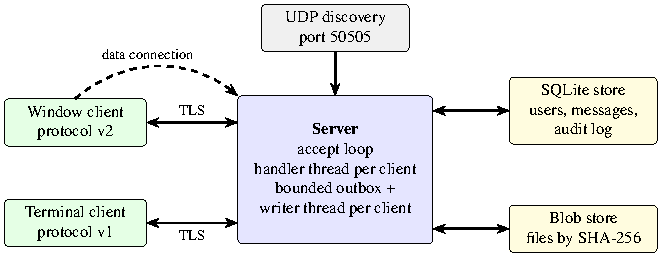
\includegraphics[width=\textwidth]{fig_architecture}
\caption{Architecture of \lch{}. Both client kinds hold one TLS connection to a central relay; file bytes use a second, short-lived data connection authorised by a ticket from the first}
\label{fig:arch}
\end{figure}

\subsection{Framing, Versions and Concurrency}
Every message in both directions is a four-byte big-endian length followed by UTF-8 text; zero-length and over-long (above 4096 bytes) frames close the connection. Version 1 carries plain text lines and is what the terminal client speaks. Version 2 carries one JSON object per frame with a type field (message, edit, reaction, presence, search, upload, key and room events and so on). The server renders every event for version-1 clients as the line they have always seen, so features were added without breaking the older client (G2).

Each connection has a handler thread that reads requests and a writer thread that is the only code writing to that socket. Delivering a message means placing it on every recipient's bounded outbound queue (100 entries) without waiting. If a queue fills, the client is not keeping up and is disconnected; it can reconnect and replay history from the database (G3). Clients ping every ten seconds; a connection silent for thirty is dropped.

\subsection{Persistence, Features and Bulk Transfer}
Messages, users, reactions, pins, read markers, sessions, public keys and the audit log live in SQLite, so history survives restarts; seven numbered migrations let an older database upgrade in place. A joining client receives the last 50 messages and can page back, and search uses an FTS5 index.

Pictures, documents and audio travel on a separate connection, as in FTP \cite{rfc959}, so that a large transfer never blocks the chat. The client announces the name, size and SHA-256; the server checks role, type, size, quota and conversation and replies with a one-time ticket. The client opens a second TLS connection, presents the ticket and streams raw bytes; the server hashes while writing a temporary file, enforces the declared size and a deadline, and only then stores the file under its hash and posts the message. A damaged file is never delivered, a half-finished upload leaves nothing behind, file names are reduced to a safe base name and executable types are blocked.

\subsection{Transport, Account and Audit Controls}
TLS 1.2 or newer protects both connections. The server generates a self-signed certificate and the client pins its fingerprint on first connect, as SSH does for host keys \cite{rfc4251}; a changed fingerprint blocks the connection. Following authentication guidance \cite{nist63b}, passwords are hashed with scrypt ($N=2^{14}$, $r=8$, $p=1$, random 16-byte salt), must be at least six characters and not a common password, and five failed sign-ins lock an account for 30 seconds, doubling to 15 minutes. A token bucket limits each user (a burst of 30 messages per ten seconds), and each address is limited to 240 connections a minute and 10 sign-ups an hour. Saved sign-ins last 12 hours and only their hash is stored. Roles (administrator, member, guest) are checked on the server for every action. Administrative actions are appended to an audit log in which each record contains the hash of the previous one, so editing the middle of the log breaks the chain and a separate head marker exposes truncation \cite{schneier99,crosby09}.

\subsection{End-to-End Encryption}
\label{sec:e2ee}

\runinhead{Identities and trust.} Each person has an X25519 key pair for key agreement and an Ed25519 pair for signatures, bound by a self-signature \cite{rfc7748,rfc8032}. Secret keys are wrapped on disk with ChaCha20-Poly1305 \cite{rfc8439} under a key derived by scrypt \cite{rfc7914} from a passphrase. A 24-character recovery code (about 119 bits) wraps a second copy that the server stores as an opaque backup. Because the server may lie about keys, clients verify each bundle's signature, pin the first key seen for each contact, block sending when it changes until the person accepts the new one, and offer a 60-digit safety number for comparison in person or on a trusted call.

\runinhead{Private messages and files.} The sender encrypts the text under a random key with ChaCha20-Poly1305, seals that key separately for the recipient and for themselves (ephemeral X25519 and HKDF-SHA256 \cite{rfc5869}), and signs the message with Ed25519, binding the sender and recipients into the authenticated data. The server stores an empty body and the envelope. Files are encrypted on the sender's computer in 64\,KiB chunks; each nonce carries the chunk number and a last-chunk flag, so dropped, reordered or added chunks fail. The key, name and type travel inside the encrypted message, so the server stores unreadable bytes under an opaque name.

\runinhead{The group room.} A sealed copy of every message for every member does not scale, so each member holds a random chain key per \emph{epoch}, derives the key for message $n$ by $n$ one-way hash-based message authentication (HMAC) steps, and gives every other member a sealed copy of the chain as it stands. A member who joins later therefore reads only what follows. The server stores the sealed copies, enforces strictly increasing message numbers per sender, and starts a new epoch whenever someone is removed or an administrator asks; the removed person never receives the new chain.

\runinhead{Key lifecycle and what the server learns.} Keys can be rotated (old identities are kept so earlier messages still open), restored from the recovery code on a new computer, or reset, which discards history; an idle window locks itself and forgets the keys. The server still sees who talks to whom, when, the sizes of messages and files, reactions, mentions, roles and room membership. There is no forward secrecy, identity is only as strong as the comparison of safety numbers, and there is one active device per person; these limits bound every confidentiality claim here.

\section{Implementation}
\label{sec:impl}
The core uses only the Python standard library \cite{pysocket,pythreading}: \code{sqlite3} and \code{hashlib} supply storage and scrypt, and \code{tkinter} supplies the desktop window. Three third-party packages are optional: \code{cryptography} for end-to-end encryption, Pillow for previews and \code{sounddevice} for voice; without the first the chat works over TLS only and the window says so (G1). The code is about 10,600 lines: 4,800 non-graphical in 21 modules, 4,900 for the window in seven and 900 for encryption in three. 

\section{Evaluation}
\label{sec:eval}
\subsection{Set-up and Correctness Tests}
All measurements were taken on one Apple-silicon laptop (arm64) running macOS 27.2 with CPython 3.14.9, with the server in one process and the load generators in separate processes on the loopback interface. Unless stated, each setting was repeated and we report the mean $\pm$ standard deviation. The repository holds 22 test modules with 453 tests, each starting real servers; they cover framing, both protocols, the database, TLS and pinning, file transfer, lockout, the audit chain and the encryption code, which is checked against published test vectors for X25519 and Ed25519 \cite{rfc7748,rfc8032} and then against tampering, forged senders, replays and the room's rules for late joiners and removal. Eleven scripts drive the real window through 370 checks.

\subsection{Fan-Out Latency and Comparison with Other Servers}

\begin{table}[!tb]
\caption{Broadcast latency, CPU time and peak resident memory by server and number of receivers (loopback; mean $\pm$ standard deviation of 8 trials, 5 for TLS and 200 receivers; every message reached every receiver in every trial)}
\label{tab:fanout}
\footnotesize
\setlength{\tabcolsep}{3pt}
\begin{tabular}{p{1.4cm}p{2.5cm}p{1.8cm}p{1.8cm}p{1.0cm}p{1.5cm}}
\svhline\noalign{\smallskip}
Receivers & Server & Median (ms) & p95 (ms) & CPU (s) & Memory (MB) \\
\noalign{\smallskip}\svhline\noalign{\smallskip}
100 & Sequential relay & 1.60 $\pm$ 0.19 & 3.35 $\pm$ 0.25 & 0.11 & 35 \\
 & asyncio relay & 2.32 $\pm$ 0.13 & 4.40 $\pm$ 0.28 & 0.21 & 33 \\
 & asyncio + SQLite & 2.98 $\pm$ 0.22 & 4.75 $\pm$ 0.43 & 0.24 & 34 \\
 & LANChat-H & 6.89 $\pm$ 0.18 & 8.84 $\pm$ 0.25 & 4.40 & 54 \\
\hline
100 (TLS) & LANChat-H & 7.32 $\pm$ 0.09 & 9.68 $\pm$ 0.51 & 4.48 & 59 \\
200 & LANChat-H & 10.14 $\pm$ 0.37 & 14.39 $\pm$ 1.77 & 9.56 & 62 \\
\noalign{\smallskip}\svhline\noalign{\smallskip}
\end{tabular}
\end{table}
One sender sent 60 messages of about 100 bytes at ten per second to $N$ receivers; latency is the arrival time minus the send time on the machine's monotonic clock. For comparison we wrote three minimal relays that speak the same wire protocol: a \emph{sequential relay} (thread per client, blocking send to each recipient in turn), an \emph{asyncio relay} (one event loop with a bounded queue and writer task per client) and an \emph{asyncio relay with SQLite} that stores every message first. They check no accounts, roles or rate limits, so they show a lower bound for each design, not a like-for-like product.


Table~\ref{tab:fanout} shows a small spread between trials (a standard deviation of at most 0.4\,ms for the median). With 100 receivers the median for \lch{} is 6.9\,ms, against 2.3\,ms for the \code{asyncio} relay (4.3\,ms against 1.0\,ms in our ten-receiver runs). The difference is \lch{}'s per-message work (role and rate checks, storage, mentions, two protocol versions); it shows in CPU time (4.4\,s over a ten-second run with 100 receivers against 0.2\,s) and memory (54\,MB against 33\,MB). TLS added about 0.4\,ms. At 200 receivers the server used 9.6\,s of CPU in a run of about ten seconds, so the thread-per-client design saturates one core at roughly 200 receivers sending ten messages a second; beyond that an \code{asyncio} or multi-process design would be needed, and we do not claim that this server scales further.

\subsection{Head-of-Line Blocking}
With sequential sends, recipient $k$ receives a message after the time given by Eq.~(\ref{eq:seq}),
\begin{equation}
D_k = \sum_{j=1}^{k} s_j ,
\label{eq:seq}
\end{equation}
where $s_j$ is the time of the blocking send to recipient $j$, and if recipient $m$ stalls for an extra time $W$ then, by Eq.~(\ref{eq:stall}),
\begin{equation}
D_k \ge W + \sum_{j=1}^{k} s_j \qquad \mbox{for all } k \ge m .
\label{eq:stall}
\end{equation}
With a bounded queue and writer thread the send to each recipient reduces to an enqueue with cost $q_j \ll W$, so $D_k$ no longer depends on $W$ for $k \neq m$. To test this, ten receivers read normally while one more connected first, shrank its receive buffer to 4\,KiB and never read; a sender sent 600 messages of 2000 bytes at 50 per second. Once the kernel buffers of the stalled connection were full, after 232 messages, the sequential relay stopped delivering to every receiver: in all ten trials exactly 2320 of the 5370--5400 expected deliveries arrived (median 0.7\,ms). \lch{} and both \code{asyncio} relays delivered 6000 of 6000 in all ten trials (median 4.0, 1.0 and 1.6\,ms for \lch{}, the \code{asyncio} relay and the \code{asyncio} relay with SQLite), so the isolation comes from the bounded queue, not from threads or from our code in particular. \lch{} also dropped the stalled connection once its queue filled, in all ten trials.



\subsection{Mixed Workload and Emulated Network Path}

\begin{table}[!tb]
\caption{Mixed workload over TLS with all limits on (60\,s; emulated one-way delay $\pm$ jitter in ms; times in ms except the upload)}
\label{tab:workload}
\footnotesize
\setlength{\tabcolsep}{3pt}
\begin{tabular}{p{1.3cm}p{1.8cm}p{1.2cm}p{1.2cm}p{1.2cm}p{2.0cm}p{1.2cm}}
\svhline\noalign{\smallskip}
Clients & Delay & Median & p95 & p99 & 1\,MB upload (s) & CPU (s) \\
\noalign{\smallskip}\svhline\noalign{\smallskip}
40 & 0 $\pm$ 0 & 4.8 & 6.7 & 7.9 & 0.02 & 4.2 \\
40 & 100 $\pm$ 20 & 207.4 & 253.8 & 272.6 & 1.08 & 4.4 \\
100 & 0 $\pm$ 0 & 6.8 & 10.6 & 14.1 & 0.02 & 15.9 \\
\noalign{\smallskip}\svhline\noalign{\smallskip}
\end{tabular}
\end{table}
Because people do not chat at a regular rate, we also ran a mixed workload with all limits and TLS on: 40 clients (100 in the last row), each sending a message after an exponentially distributed pause (mean 6\,s) with a log-normal size (median about 60 bytes) and the usual heartbeat, while one more client uploaded a 1\,MB file every 5 seconds. A small user-space proxy emulated a network path by delaying each direction by a base time plus Gaussian jitter; it cannot create packet loss, which TCP hides as extra delay.


Every message reached every receiver in all six runs (Table~\ref{tab:workload} shows three). With no added delay the median was about 5\,ms with 40 clients and 7\,ms with 100. With an added one-way delay $d$ it grew to about $2d+7$\,ms, so the server added a roughly constant 7--8\,ms on top of the two crossings of the path, and the upload time grew with the round trips of the ticket exchange. This is an emulation, not a measurement of Wi-Fi or Ethernet; we have not yet run our probe script across real devices.

\subsection{Cost of Security Operations and File Transfer}
Medians over 30 runs, with a standard deviation under 10\% of the median, were: a password check 28.6\,ms by design, as the price of making offline guessing expensive; wrapping the keys with a passphrase 59.6\,ms; a safety number 2.1\,ms; encrypting and decrypting a 200-byte message for one person 0.30 and 0.25\,ms; a room message 0.16 and 0.25\,ms; and a 20\,MB file 29.9\,ms to encrypt (about 670\,MB/s) and 20.2\,ms to decrypt, so the cost of end-to-end encryption is dominated by passphrase stretching, not by the ciphers. Over loopback the file path reached 270--820\,MB/s for uploads and 570--1030\,MB/s for downloads without TLS, and roughly 55--80\% of that with TLS.



\subsection{Confidentiality Check and Our Own Security Testing}
The confidentiality claim of G5 is checked by observation. A test records every frame the server receives or sends while two people exchange a private message, an edit, a room message and an encrypted file, and scans the frames, the SQLite file and the stored files for the secret texts, the real file name, the file contents and the keys. None appears, although the encrypted envelopes do; a companion check shows that the same capture finds a plaintext message.

We also tested the server as an attacker would, with tools we wrote ourselves; \emph{this is not independent testing}. Twenty seeded fuzzing runs sent about 29,600 hostile connections before sign-in, about 160,000 mutated events after sign-in (every event type, with hostile field values) and 4,000 made-up transfer tickets. The first version found one real bug: an integer above $2^{63}$ reached SQLite and ended the sender's connection thread. We now refuse such a request and keep the connection, with a regression test; the final runs found no unhandled exception. A TLS probe showed that the server refuses TLS 1.0 and 1.1 and accepts 1.2 and 1.3. A static scan reported no high-severity finding; of ten medium findings, three are the intended bind to all interfaces and seven are queries built only from fixed fragments and placeholders, which we checked by hand.

\subsection{Threats to Validity}
All measurements come from one machine and one Python version over loopback, so a real network, wireless loss and a second device are absent, and the emulated delay is not a real path. The trials give a tight spread but are not a statistical study, and the mixed workload was run once per setting. The baselines are minimal relays, not other chat products. The security testing was written and run by the authors: it shows that these inputs are handled, not that no input breaks the system.

\section{Discussion and Limitations}
\label{sec:discussion}
A renderer that turns every event into the line an older client expects made incremental growth cheap, and testing against real servers and the real window found problems that tests of pieces would not, such as the oversized-integer bug above and an invisible recovery-code button. End-to-end encryption is less about the cipher than about everything the server used to do with plaintext: search, pins, mentions and moderation each needed a client-side or metadata-based replacement.

The main limits are these. There is \emph{no forward secrecy}: theft of a recipient's long-term key would expose earlier messages to anyone holding the ciphertext, and the room's sealed chain copies stay on the server so that history can be re-read; a ratchet \cite{signal,cohngordon} would be the upgrade. Keys are pinned on first sight, but until two people compare security codes a hostile server could have substituted a key at first contact, and the same holds for the server certificate under trust on first use. The server learns who talks to whom and when, sizes and mentions, and administrators cannot moderate by reading. Terminal clients and members without keys cannot take part in encrypted conversations, search of encrypted messages covers only what the window has loaded, and files in readable conversations are stored unencrypted. Finally, the server saturates a core at about 200 receivers; we did not build a full \code{asyncio} version of \lch{} \cite{pyasyncio}, so how much of its feature cost would remain is untested. Future work includes a ratchet, multiple devices per person, protection of metadata, an asynchronous server with the full feature set, measurements over real networks and an independent security review.

\section{Conclusion}
\label{sec:conclusion}
\lch{} shows that a chat system for a local network can combine a compatible protocol, isolation of slow clients, layered transport and account security, and end-to-end encryption for private conversations and an optional group room, in a code base small enough to read and with one optional dependency. The measurements show the price: a few milliseconds of extra per-message work for a room that survives a stalled receiver, and a fraction of a millisecond per encrypted message for a server that holds only ciphertext. The limits are stated plainly: no forward secrecy, visible metadata, trust on first use, a single-core ceiling near 200 receivers, and measurements and security testing that come from one machine and from the authors.



\begin{thebibliography}{99.}
\bibitem{rfc9293} Eddy, W. (ed.): Transmission Control Protocol (TCP). RFC 9293, IETF (2022)
\bibitem{pysocket} Python Software Foundation: socket -- Low-level networking interface. Python 3 Documentation. \url{https://docs.python.org/3/library/socket.html} (accessed 2026)
\bibitem{pythreading} Python Software Foundation: threading -- Thread-based parallelism. Python 3 Documentation. \url{https://docs.python.org/3/library/threading.html} (accessed 2026)
\bibitem{saltzer} Saltzer, J.H., Reed, D.P., Clark, D.D.: End-to-end arguments in system design. ACM Trans. Comput. Syst. 2(4), 277--288 (1984)
\bibitem{rfc1459} Oikarinen, J., Reed, D.: Internet Relay Chat Protocol. RFC 1459, IETF (1993)
\bibitem{rfc6120} Saint-Andre, P.: Extensible Messaging and Presence Protocol (XMPP): Core. RFC 6120, IETF (2011)
\bibitem{rfc6455} Fette, I., Melnikov, A.: The WebSocket Protocol. RFC 6455, IETF (2011)
\bibitem{seda} Welsh, M., Culler, D., Brewer, E.: SEDA: an architecture for well-conditioned, scalable Internet services. In: Proceedings of the 18th ACM Symposium on Operating Systems Principles (SOSP 2001), pp. 230--243. ACM, New York (2001)
\bibitem{lee} Lee, E.A.: The problem with threads. Computer 39(5), 33--42 (2006)
\bibitem{rfc8446} Rescorla, E.: The Transport Layer Security (TLS) Protocol Version 1.3. RFC 8446, IETF (2018)
\bibitem{signal} Perrin, T., Marlinspike, M.: The Double Ratchet Algorithm, Revision 1. Signal (2016). \url{https://signal.org/docs/specifications/doubleratchet/}
\bibitem{cohngordon} Cohn-Gordon, K., Cremers, C., Dowling, B., Garratt, L., Stebila, D.: A formal security analysis of the Signal messaging protocol. In: Proceedings of the IEEE European Symposium on Security and Privacy (EuroS\&P 2017), pp. 451--466. IEEE (2017)
\bibitem{x3dh} Marlinspike, M., Perrin, T.: The X3DH Key Agreement Protocol, Revision 1. Signal (2016). \url{https://signal.org/docs/specifications/x3dh/}
\bibitem{rfc9420} Barnes, R., Beurdouche, B., Robert, R., Millican, J., Omara, E., Cohn-Gordon, K.: The Messaging Layer Security (MLS) Protocol. RFC 9420, IETF (2023)
\bibitem{unger} Unger, N., Dechand, S., Bonneau, J., Fahl, S., Perl, H., Goldberg, I., Smith, M.: SoK: Secure messaging. In: Proceedings of the IEEE Symposium on Security and Privacy (SP 2015), pp. 232--249. IEEE (2015)
\bibitem{matrix} The Matrix.org Foundation: Matrix Specification. \url{https://spec.matrix.org} (accessed 2026)
\bibitem{omemo} XMPP Standards Foundation: XEP-0384: OMEMO Encryption. \url{https://xmpp.org/extensions/xep-0384.html} (accessed 2026)
\bibitem{rfc959} Postel, J., Reynolds, J.: File Transfer Protocol (FTP). RFC 959, IETF (1985)
\bibitem{rfc4251} Ylonen, T., Lonvick, C. (eds.): The Secure Shell (SSH) Protocol Architecture. RFC 4251, IETF (2006)
\bibitem{nist63b} Grassi, P.A., Garcia, M.E., Fenton, J.L.: Digital Identity Guidelines: Authentication and Lifecycle Management. NIST Special Publication 800-63B (2017). \url{https://doi.org/10.6028/NIST.SP.800-63b}
\bibitem{schneier99} Schneier, B., Kelsey, J.: Secure audit logs to support computer forensics. ACM Trans. Inf. Syst. Secur. 2(2), 159--176 (1999)
\bibitem{crosby09} Crosby, S.A., Wallach, D.S.: Efficient data structures for tamper-evident logging. In: Proceedings of the 18th USENIX Security Symposium, pp. 317--334. USENIX Association, Berkeley (2009)
\bibitem{rfc7748} Langley, A., Hamburg, M., Turner, S.: Elliptic Curves for Security. RFC 7748, IETF (2016)
\bibitem{rfc8032} Josefsson, S., Liusvaara, I.: Edwards-Curve Digital Signature Algorithm (EdDSA). RFC 8032, IETF (2017)
\bibitem{rfc8439} Nir, Y., Langley, A.: ChaCha20 and Poly1305 for IETF Protocols. RFC 8439, IETF (2018)
\bibitem{rfc7914} Percival, C., Josefsson, S.: The scrypt Password-Based Key Derivation Function. RFC 7914, IETF (2016)
\bibitem{rfc5869} Krawczyk, H., Eronen, P.: HMAC-based Extract-and-Expand Key Derivation Function (HKDF). RFC 5869, IETF (2010)
\bibitem{pyasyncio} Python Software Foundation: asyncio -- Asynchronous I/O. Python 3 Documentation. \url{https://docs.python.org/3/library/asyncio.html} (accessed 2026)
\end{thebibliography}

\end{document}
